\documentclass[fleqn]{report}
\usepackage{geometry}
\usepackage{amssymb}
\usepackage{fancyhdr}
\usepackage{multicol}
\usepackage{blindtext}
\usepackage{color}
\usepackage[fontsize=16pt]{fontsize}
\usepackage{lipsum}
\usepackage{pgfplots}
\usepackage{physics}
\usepackage{mathtools}
\usepackage[makeroom]{cancel}
\usepackage{ulem}
\usepackage{esint}

\graphicspath{ {../Images/} }
\setlength{\columnsep}{1cm}
\addtolength{\jot}{0.1cm}
\def\columnseprulecolor{\color{blue}}
\date{Spring 2025}

\newcommand{\textoverline}[1]{$\overline{\mbox{#1}}$}

\newcommand{\hp}{\hspace{1cm}}

\newcommand{\const}{\textrm{const}}

\newcommand{\del}{\partial}

\newcommand{\pdif}[2]{ \frac{\partial #1}{ \partial #2} }

\newcommand{\pderiv}[1]{ \frac{\partial}{ \partial #1} }

\newcommand{\comment}[1]{}

\newcommand{\equations} [1] {
\begin{gather*}
#1
\end{gather*}
}

\newcommand{\numequations} [1] {
\begin{gather}
#1
\end{gather}
}

\newcommand{\twovec}[2]{ 
\begin{pmatrix}
#1 \\ 
#2
\end{pmatrix}
}

\title{PHYS 435}
\author{Aiden Sirotkine}

\begin{document}

\pagestyle{fancy}
\maketitle
\tableofcontents
\clearpage

\chapter{PHYS435}
This goddamn professor is half retired im so cooked 

\section{Coulomb's Law}
\equations{
    \vec E(\vec r) = \frac{1}{4 \pi \epsilon_0} \frac{q}{r^2} \hat r 
    \\
    \vec E(\vec r) = \sum \frac{1}{4 \pi \epsilon_0} \frac{q}{r^2} \hat r 
    \rightarrow 
    \frac{1}{4 \pi \epsilon_0} 
    \int 
    d^3 r' 
    \frac{\vec r - \vec r'}{|\vec r - \vec r'|^3} \rho(\vec r')
}

\section{Gauss's Law}
The flux of $\vec E$ throuhg a closed surface equations to the enclosed charge $C_0$

\equations{
    \frac{1}{C_0} \int_V d^3 r \rho(\vec r) = \int_{\del V} d a \rho(\vec r)
}

\section{Divergence Theorem}
\equations{
    \vec \nabla E = \del_x E_x + \del_y E_y + \del_z E_z
    \\
    \int_V d^3 r \vec \nabla \vec E(\vec r) = \int_{\del V} d \vec a \cdot \vec E(\vec r)
    \\
    \vec \nabla \vec E(\vec r) = \frac{\rho(\vec r)}{\epsilon_0}
}

\section{Faraday's Law}
The circulation of $\vec E$ around any closed path $N$ is equal to $(-1) \times$ 
the time derivative of the magnetic flux  through ANY surface bounded by 
the closed path.

\equations{
    \int_{\del S} d \vec l \cdot \vec E = - \frac{d}{dt} \int_S d \vec a \vec B 
}

\section{Stoke's Theorem}
\equations{
    \int_{\del S} d \vec l \cdot \vec E = 
    \int_S d \vec a \vec \nabla \times \vec E 
}

\subsection{Differential Laws}
\equations{
    \vec \nabla \times \vec E = - \frac{\del}{\del t} \vec B 
    \\
    \textrm{Gauss}
    \\
    \vec \nabla \cdot \vec E = - \frac{\rho(\vec r)}{\epsilon_0}
    \hp 
    \vec \nabla \cdot \vec B = 0
    \\
    \textrm{Ampere}
    \\
    \vec \nabla \times \vec B = \mu_0 J
}

\section{Electric Potential}
Start with Maxwell's Equations
\equations{
    \vec \nabla \cdot \vec E(\vec r) = \frac{ \rho(\vec r)}{\epsilon_0}
    \\
    \vec \nabla \times \vec E(\vec r) = - \frac{\del}{\del t} \vec B(\vec r, t)
    \\
    \vec \nabla \cdot \vec B(\vec r) = 0
    \\
    \vec \nabla \times \vec B = 
    \mu_0 \vec J + \mu_0 \epsilon_0 \frac{\del}{\del t} \vec E
}
remove the time dependent equations 
\equations{
    \vec \nabla \cdot \vec E(\vec r) = \frac{ \rho(\vec r)}{\epsilon_0}
    \\
    % \vec \nabla \cdot \vec B(\vec r) = 0
    % \\
    \vec \nabla \times \vec E(\vec r) = 0
}
the curl of $\vec E$ is 0 which means the electric field is conservative? 
A scalar potential function convenience.

consider the path integral 
\equations{
    \int\limits_P d \vec l \cdot \vec E 
}
We can show that the integral is path independent (because the curl is 0)
\equations{
    \int\limits_{P1} - \int\limits_{P2} = 
    \oint\limits_{\del S} d \vec l \cdot \vec E(\vec r)
    =
    \int\limits_S d \vec a \cdot \vec \nabla \times \vec E
    = 0
    \\
    \int\limits_{P1} d \vec l \cdot \vec E = \int\limits_{P2} d \vec l \cdot \vec E
}
That's actually a really smart proof damn 

Now we do actual potential stuff 
\equations{
    V(\vec r) = - \int^{\vec r}_{\vec 0_r} d \vec l \cdot \vec E(\vec r)
}
Where $\vec 0_r$ is the vector where the potential is 0
\equations{
    U(\vec a) - U(\vec b) = - \int^b_a d \vec l' \cdot \vec F(\vec r)
    \\
    \vec F_{Lorentz} = q \vec E(\vec r) + q \vec v(\vec r) \times \vec B(\vec r)
}
$q \vec E(\vec r)$ can do work, but $q \vec v(\vec r) \times \vec B(\vec r)$ 
cannot do any work (always in opposite direction of motion)

\equations{
    W 
    =
    q \int^{\vec r}_{\vec 0_{r}} d \vec l \cdot 
    \vec v \times \vec B 
    = 
    q \int^{\vec r}_{\vec 0} d \vec l \cdot 
    \frac{d \vec l}{dt} \times \vec B(\vec r)
    =
    \\
    q \int^{\vec r}_{\vec 0} dt \frac{d \vec l}{dt} \cdot 
    (\frac{d \vec l}{dt} \times \vec B(\vec r))
    = 0
}
That part cannot do any work 
\equations{
    W_{other} = U(\vec r) - U(\vec 0)
    \\
    \frac{U(\vec r) - U(\vec 0)}{q} = \Delta V
}
More Stuff 
\equations{
    V(\vec r) = - \int^{\vec r}_{\vec 0_r} d \vec l' \cdot \vec E(\vec r)
    \\
    - \vec \nabla V(\vec r) 
    =
    -
    \left[
        \hat x \frac{\del}{\del x} V(\vec r) + 
        \hat y \frac{\del}{\del y} V(\vec r) +
        \hat z \frac{\del}{\del z} V(\vec r)
    \right]
    \\
    d \vec r = \hat x dx + \hat y dy + \hat z dz 
    =
    r + dx 
}
consider the slightest motion $dx$ in the $\hat x$ direction so that 
$\vec r \to \vec r + \hat x dx$
\equations{
    V(\vec r + \hat x dx) = V(\vec r) + dx \hat x \cdot \vec E(\vec r)
    \hp 
    E_x(\vec r) = \hat x \cdot \vec E(\vec r)
    \\
    \frac{V(\vec r + \hat x dx) - V(\vec r)}{dx} = E_x(\vec r)
}
That gives us 
\[
\vec E(\vec r) = - \nabla V(\vec r)
\]
real important equation 

\subsection{Potential Equation}
consider a point mass 
\equations{
    \vec E(\vec r) = 
    \frac{1}{4 \pi \epsilon_0} q \frac{\vec r}{r^3} = 
    \frac{1}{4 \pi \epsilon_0} \frac{q}{r^2} \hat r
    \\
    V(\vec r) = - \int^{\vec r}_{\vec 0_r} d \vec l \cdot \vec E 
    \\
    E_y = \frac{1}{4 \pi \epsilon_0} \frac{q}{y^2}
    \hp 
    - \int^y_\infty dy' \frac{1}{4 \pi \epsilon_0} \frac{q}{y^2}
    \\
    V(\vec r) = \frac{1}{4 \pi \epsilon_0} \frac{q}{r}
}
Use the principle of superposition to get the general answer 
\equations{
    V(\vec r) = \frac{1}{ 4 \pi \epsilon_0} 
    \int d^3 r' \frac{\rho(\vec {r'})}{|\vec r - \vec {r'}|}
}

\subsection{Infinite Line Charge}
Consider a straight line of infinite length and constant charge density. 

Where should $\vec 0_{r}$ be?

I think we just pick an arbitrary point 

\equations{
    \vec E(s) = \frac{\lambda}{2 \pi \epsilon_0} \frac{1}{s}
    \\
    V(\vec r) = - \int d \vec l \vec E(s) = V(s) = 
    - \int^s_{O_r} ds \frac{1}{2 \pi \epsilon_0} \frac{\lambda}{s'}
    \\
    =
    - \frac{\lambda}{2 \pi \epsilon_0} \ln(s') \Big|^s_{\vec O_r}
    =
    \frac{\lambda}{2 \pi \epsilon_0} \ln(\frac{O_r}{s})
}

What PDE governs $V(\vec r)$

\equations{
    \vec \nabla \cdot \vec E = \frac{\rho}{\epsilon_0}
    \hp 
    \vec E = - \vec \nabla V 
    \\
    \vec \nabla \cdot \vec \nabla V(\vec r) = -\frac{\rho}{\epsilon_0}
    \\
    (\del_x^2 + \del_y^2 + \del_z^2) V = -\frac{\rho}{\epsilon_0}
    \\
    \nabla^2 V(\vec r) = -\frac{\rho(\vec r)}{\epsilon_0}
}


\section{Work}
If you move 1 charge, there is no work done because there are no other 
fields. 

If you bring in a 2nd charge, you get a total work of 
$
\frac{1}{4 \pi \epsilon_0} \frac{q_1 q_2}{|\vec r_1 - \vec r_2|}
$

If you bring in a third charge you just sum the things together 

\equations{
    U_{1 \to N} = \frac{1}{2} \sum^N_i \sum^N_{j > i} 
    \frac{1}{4 \pi \epsilon_0} \frac{q_i q_j}{|\vec r_i - \vec r_j|}
    =
    \frac{1}{2} \int d^3 r d^3 r' \frac{1}{4 \pi \epsilon_0} 
    \frac{\rho(\vec r) \rho(\vec{r'})}{|\vec r - \vec{r'}|}
    \\
    =
    \frac{1}{2} \frac{1}{4 \pi \epsilon_0} 
    \int d^3 r' \rho(\vec{r'}) V(\vec{r'})
    \hp 
    \rho(\vec{r'}) = - \epsilon_0 \nabla^2 V(\vec{r'})
    \\
    U = - \frac{\epsilon_0}{2} \int d^3 r V(\vec r) \nabla^2 V(\vec r)
}

\subsection{X-component}
Let's consider just the $x$-component for a little bit 

\equations{
    - \frac{\epsilon_0}{2} 
    \int d^3 r V(\vec r) \del_x \left[ \del_x V(\vec r) \right]
    \\
    \del_x \left[ V(\vec r) \del x V(\vec r) \right]
    =
    \del_x V \cdot \del_x V + V \del_x^2 V 
    \\
    \del_x \left[ V(\vec r) \del x V(\vec r) \right]
    - \del_x V \cdot \del_x V 
    =
    V \del_x^2 V 
}
So with that you get 
\equations{
    - \frac{\epsilon_0}{2} 
    \int d^3 r V(\vec r) \del_x \left[ \del_x V(\vec r)\right]
    =
    - \frac{\epsilon_0}{2} 
    \int d^3 r \del_x \left( V(\vec r) \del_x V (\vec r)\right)
    - E_x^2
}
generalize 
\equations{
    \frac{\epsilon_0}{2} 
    \int d^3 r \, \vec \nabla \cdot V(\vec r) \vec E(\vec r) + 
    \vec E \cdot \vec E 
}

The main point of all of this is that it goes to $0$ for large $r$ 
\equations{
    \int d^3 r \vec \nabla \cdot V \vec E 
    \rightarrow 
    \int d^3 r \vec \nabla \cdot \frac{C}{r} \frac{1}{r^2} \hat r 
    \rightarrow 
    \\
    \int da \frac{C}{r^3}
    \rightarrow 
    \frac{1}{r}
    \rightarrow \lim_{r \to \infty} = 0
}

So our potential somehow gets to 
\equations{
    U  =
    \int d^3 r \frac{\epsilon_0}{2} E^2 
}

\section{Office Hours Math}
So using Gauss's Law we can say that the net charge around the eye 
sockets is 0

\equations{
    \phi_E = 
    \frac{Q_{enc}}{\epsilon_0}
    =
    \oiint E dA
}

If we consider 
\equations{
    V = \frac{1}{4 \pi \epsilon_0} \frac{q}{r}
}
where $r$ is the surface of the thing. 

Basically the locations of all the things makes sense 

\section{More Energy}
So we spent all of last lecture getting 
\equations{
    U_E(\vec r) = \frac{\epsilon_0}{2} E^2
    \\
    U_{b \to c}
    =
    \int r^2 dr \sin(\theta) d \theta d \phi \frac{\epsilon_0}{2} 
    \frac{Q^2}{(4 \pi \epsilon_0)^2} \frac{1}{r^4}
    \\
    =
    \frac{Q^2}{8 \pi \epsilon_0} \int^c_b \frac{r^2}{r^4} dr 
    =
    \frac{Q^2}{8 \pi \epsilon_0} 
    \left(
        \frac{1}{b}
        -
        \frac{1}{c}
    \right)
}

\section{Dirac Delta}
Consider a Gaussian curve given by 
\equations{
    G(x) = Ge^{\frac{-x^2}{a^2}}
    =
    \frac{1}{a \sqrt{\pi}} e^{\frac{-x^2}{a^2}}
    \\
    \int \, dx
    \frac{1}{a \sqrt{\pi}} e^{\frac{-x^2}{a^2}}
    = 1
    \\
    \delta(X) = 
    \lim_{a \to 0}
    \frac{1}{a \sqrt{\pi}} e^{\frac{-x^2}{a^2}}
}
The integral is 1, but all of the area is located at the point $x = 0$
\equations{
    \delta(x - x_0) =
    \lim_{a \to 0}
    \frac{1}{a \sqrt{\pi}} e^{\frac{-(x - x_0)^2}{a^2}}
}
\equations{
    \int^{\infty}_{-\infty}
    dx \delta(x - x_0)
    = 1
    \\
    \int^{\infty}_{-\infty}
    dx \delta(x - c) f(x)
    = f(c)
    \\
    \rho(\vec r) = q \delta(x - x') \delta(y - y') \delta(z - z')
}

\chapter{Conductors and Surfaces}
The electric field at the surface of a plane is 
\equations{
    E_{\perp} = \frac{1}{2} \frac{\sigma}{\epsilon_0}
}
Because of the surface field, there is a pressure on the surface 
\equations{
    P = E * \sigma = \frac{1}{2} \frac{\sigma^2}{\epsilon_0}
}

Given some set of conductors, there is a number that, given the potential 
at a point, can tell you the net charge in the set. 

That number is the capacitance
\equations{
    C \Delta V = Q 
}

\subsection{Parallel Plate Capacitors}
Consider 2 plates of charges $+Q$ and $-Q$. 

We can integrate the electric field to get the potential difference 
\equations{
    V = d * E = d * \frac{\sigma}{\epsilon_0}
    =
    \frac{d * Q}{\textrm{Area} * \epsilon_0} = \frac{Q}{C}
    \\
    C = \frac{\epsilon_0 A}{d}
}
Where $d$ is distance and not the differential operator

Now we can find the energy of the system 
\equations{
    U = 
    \frac{\epsilon_0}{2} 
    \frac{\sigma^2}{\epsilon_0^2}
    \frac{A^2}{A} * d
    =
    \frac{1}{2} \frac{Q^2}{\epsilon_0 A/d} 
    =
    \frac{1}{2} \frac{Q^2}{C}
}
That is the stored energy in a field. 

There's another way to get the same derivation.
\equations{
    dW = dQ \cdot V 
    \\
    \int^W_0 dW = U = \int^Q_{Q = 0} dQ V = 
    \int^Q_0 dQ \frac{Q}{C} = \frac{Q^2}{2C}
}

\subsection{Constant $Q$}
What happens if we pull part the plates of the capacitor?

$d$ goes up, $C$ goes down, $V$ goes up, $U$ goes up

\subsection{Constant $V$}
We have the parallel plate capacitor hooked up to a battery of 
constant voltage 

$d$ goes up, $C$ does down, $Q$ must go down for $V$ to not change 

The internal energy can also be written as $U = \frac{1}{2} CV$

\equations{
    dU = - \vec F \cdot dr 
}


In a volume $V$ without charges, $V(\vec r)$ has 
a maximum and minimum on $\del V$, the boundary, not inside. 

Imagine a blob with all sorts of potential and voltage and whatever 

This just gives us our definition $\del V$ = the boundary of the object 

We have the equation 
\[
\nabla^2 U(\vec r) = -\frac{\rho(\vec r)}{\epsilon_0}
\]

Let's try to figure out the average potential on the surface of the sphere 
\equations{
    V(\vec r) 
    = 
    \frac{1}{4 \pi R^2}
    \int da \, V
}

What we'll learn is that $V$(origin) = the area of $V$ on the sphere 

\equations{
    V(\vec(r')) = \frac{q}{4 \pi \epsilon_0} \frac{1}{|\vec{r'} - z \hat z|}
    \\
    \vec{r'}
    =
    R \sin(\theta) \cos(\phi) \hat x 
    +
    R \sin(\theta) \sin(\phi) \hat y 
    +
    R \cos(\theta) \hat z
    \\
    d(\theta, \phi)
    =
    \sqrt{
        R^2 \sin^2(\theta) \cos^2(\phi)
        +
        R^2 \sin^2(\theta) \sin^2(\phi)
        +
        (R \cos(\theta) - z)^2 
    }
    \\
    =
    \sqrt{R^2 + z^2 - 2 Rz\cos(\theta)}
    \\
    V(\vec{r}) 
    =
    \frac{1}{4 \pi R^2} \int da \cdot V(\vec{r'})
    \hp
    (\sin(\theta) d \theta = - d \cos(\theta))
    \\
    = \frac{q}{4 \pi \epsilon_0} \frac{2 \pi}{4 \pi} \int -d \cos(\theta)
}
Do a U-sub 
\equations{
    \frac{1}{2} \frac{q}{4 \pi \epsilon_0} 
    \int^1_{-1} du \, \frac{1}{\sqrt{R^2 + z^2 - 2 R z u}}
    \\
    =
    \frac{1}{2 R z} \frac{q}{4 \pi \epsilon_0} \sqrt{R^2 + z^2 - 2RzU} 
    \Big|^1_{-1}
    =
    R^2 + z^2 - 2 Rz
    \\
    \frac{1}{2 R z} \frac{q}{4 \pi \epsilon_0}
    \left[
        z - R - z - R
    \right]
    \\
    =
    \frac{q}{4 \pi \epsilon_0} \frac{1}{z}
}

\section{Surface Potential}
Where there is no charge, what is the max + min of $V(\vec r)$ on $\del V$ the 
boundary 

\section{Dirichlet Problems}
Consider an aribitrary blob with some potential 

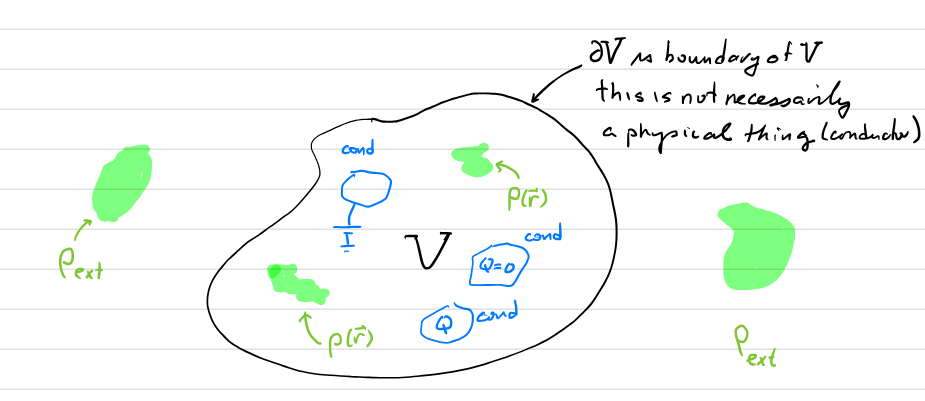
\includegraphics[width = 16cm, height = 10cm]{PHYS435.1.png}

If given $V(\vec r)$ on $\del V$ and the charge density $\rho(\vec r)$
, then $V(\vec r)$ inside the blob is uniquely determined. 

consider $V_1(\vec r)$ and $V_2(\vec r)$ such that 
\equations{
    \nabla^2 V_1 = - \frac{\rho}{\epsilon_0}
    \hp 
    V_1(\vec r) \textrm{ on } \del V = B_s(\vec r)
    \\
    \nabla^2 V_2 = - \frac{\rho}{\epsilon_0}
    \hp 
    V_2(\vec r) \textrm{ on } \del V = B_s(\vec r)
    \\
    V_3 = V_1 - V_2 
    \hp 
    \nabla^2 V_3(\vec r) = 0 
    \\
    V_3(\vec r) \textrm{ on } \del V = 0 
    \\
    V_3 = 0 \textrm{ everywhere in } V 
}
So $V_1 = V_2$ so they describe the same potential function so 
there's only 1 unique answer for each boundary potential and density 

\section{Neumann Problem}
Where do the charges lie on a conductor?

Consider a volume with a conducting boundary

The electric field inside the boundary is unique 

\equations{
    \vec \nabla \vec E = \frac{\rho}{\epsilon_0}
}

\section{New Lecture}
Find the solution for $V(\vec r)$ inside a volume of $V$.

Utilize a point-source response function. 
\equations{
    G(\vec r, \vec{r'})
    \Rightarrow 
    V(\vec r) 
    =
    \frac{1}{4 \pi \epsilon_0}
    \int d^3 r' \, 
    G(\vec r, \vec{r'}) \rho(\vec r)
}
So if we consider the normal potential function in free space (FS)
\equations{
    V(\vec r) = \frac{1}{4 \pi \epsilon_0} 
    \int d^3 r \,
    \frac{\rho(\vec r)}{|\vec r - \vec{r'}|}
}
We can see that 
\equations{
    G_{FS}(\vec r)
    =
    \frac{1}{|\vec r - \vec{r'}}
}
Which is just the response to a single point charge. 

Now let's consider the potential of a conducting grounded plane (GP)
\equations{
    V(\vec r) = \frac{1}{4 \pi \epsilon_0}
    \int\limits_{V} d^3 r' \, 
    G_{GP} (\vec r, \vec{r'}) \rho(\vec{r'})
}

Image solution:

If we consider equidistant point charges on 2 sides of the non-conducting plane, 
Then we electric field lines are perpendicular to the plane at the plane. 
The conducting plane ACTS equivalently to the equidistant point charge 

Back to math

\equations{
    V(\vec r) = 
    \frac{1}{4 \pi \epsilon_0}
    \int\limits_{V} d^3 r' \, 
    G_{GP} (\vec r, \vec{r'}) \rho(\vec{r'})
    \\
    =
    \frac{1}{4 \pi \epsilon_0}
    \int\limits_{V} d^3 r' \, 
    \rho(\vec{r'})
    \left[
        \frac{1}{|\vec r - \vec{r'}|}
        -
        \frac{1}{|\vec r - \vec{r''}|}
    \right]
    \hp
    \vec{r''} = \vec r - 2 \hat z(\vec{r'}, z)
    \\
    =
    \frac{1}{4 \pi \epsilon_0}
    \int\limits_{V} d^3 r' \, 
    \rho(\vec{r'})
    \left[
        \frac{1}{|\vec r - \vec{r'}|}
        -
        \frac{1}{|\vec r - \vec{r'} + 2 \hat z(\vec r, \hat z)|}
    \right]
    \\
    V(\vec r)
    =
    \\
    \frac{1}{4 \pi \epsilon_0}
    \int\limits_{V} d^3 r' \, 
    \rho(\vec{r'})
    \\
    \Big[
        \frac{1}
        { \sqrt{(x - x')^2 + (y - y')^2 + (z - z')^2} }
        \\
        -
        \frac{1}
        { \sqrt{(x - x')^2 + (y - y')^2 + (z + z')^2} }
    \Big]
}

All of those are equivalent 

There is not an actual image charge, but the plane acts like the 
image charge because the potential at the plane is 0 and 
all the electric field lines are perpendicular to the plane at the plane. 

Consider when $z = 0$
\equations{
    \vec E(x, y, z = 0)
    =
    \hat z \frac{\sigma}{\epsilon_0}
    \\
    =
    -\hat z \frac{q}{4 \pi \epsilon_0} \del_z 
    \Big(
        \frac{1}
        { \sqrt{(x - x')^2 + (y - y')^2 + (z - z')^2} }
        \\
        -
        \frac{1}
        { \sqrt{(x - x')^2 + (y - y')^2 + (z + z')^2} }
    \Big)
    \\
    \sigma 
    =
    \frac{q}{4 \pi}
    \frac{\del}{\del z}
    \Big(
        \frac{1}
        { \sqrt{(x - x')^2 + (y - y')^2 + (z - z')^2} }
        \\
        -
        \frac{1}
        { \sqrt{(x - x')^2 + (y - y')^2 + (z + z')^2} }
    \Big)
    \\
    \sigma 
    =
    \frac{-q}{2 \pi}
    \frac{z'}{(x^2 + y^2 + (z')^2)^{3/2}}
}
Because the coordinates are squared, you can swap $\vec{r}$ and $\vec{r'}$ 
and nothing changes. 

\section{Grounded Conducting Sphere}

\subsection{Exterior}
Use the law of superposition 
\equations{
    V(\vec r) 
    =
    \frac{1}{4 \pi \epsilon_0}
    \int\limits_V d^3 r' 
    \rho(\vec{r'}) G_{GS}(\vec r, \vec{r'})
}
Consider a point $a$ outside the sphere and a point $b$ inside the sphere 
and a mapping from the inside to the outside 
\equations{
    a * b  = R^2 
    \rightarrow 
    b = R \frac{R}{a}
}
This is basically just a method guess without any real backing, 
but we'll see that this mapping does work mathematically.
\equations{
    q'' = -q' * \frac{R}{a}
    \\
    V(\vec r)
    =
    \frac{q'}{4 \pi \epsilon_0}
    \left(
        \frac{1}{
            \sqrt{x^2 + y^2 + (z + a)^2}
        }
        -
        \frac{R/a}{
            \sqrt{x^2 + y^2 + (z - \frac{r^2}{a})^2}
        }
    \right)
}
The point on the sphere have a potential of $0$ 

\equations{
    \sqrt{x^2 + y^2 + (z + a)^2}
    =
    \frac{R}{a}
    \sqrt{x^2 + y^2 + (z - \frac{r^2}{a})^2}
    \Rightarrow 
    \\
    \Rightarrow 
    \Rightarrow 
    =
    (x^2 + y^2 + z^2) = R^2 
}

That means that we have in fact found our response function 
for a grounded sphere.

\equations{
    \frac{q'}{4 \pi \epsilon_0}
    \left(
        \frac{1}{|\vec r - \vec{r'}|}
        -
        \frac{R / r'}{|\vec r - \frac{R^2}{r'} \frac{\vec{r'}}{r'}}
    \right)
    \\
    V(\vec r)
    =
    \frac{q'}{4 \pi \epsilon_0}
    \int d^3 r' \, 
    \rho(\vec{r'})
    \left(
        \frac{1}{|\vec r - \vec{r'}|}
        -
        \frac{R / r'}{|\vec r - \frac{R^2}{r'} \frac{\vec{r'}}{r'}}
    \right)
}
That last bit is our Green's function. 

\subsection{Interior}
Because the sphere is grounded, there is no real 
potential on the outside of the sphere 
if the charge is on the sindie of the sphere 

The previously calculated solution works for both the inside 
and the outside of the sphere. 

The point source response function is useful because it allows you 
to consider any charged shape as a superposition of points. 
\equations{
    V = \frac{1}{4 \pi \epsilon_0}
    \int\limits_V d^3 r' G(\vec r, \vec{r'}) \rho(\vec{r'})
}

\section{Boundary Value Problems}

You have a conducting shape such that $\nabla^2 V = 0$ on the inside  
and you're trying to find the potential on the boundary. 

\subsection{Box}
Consider a box. 
We have to think of the potential on each side of the box
\equations{
    V_T(x, y, z = c)
    \hp
    V_B(x, y, z = 0)
}
Specify $V_B$

Find 
\equations{
    V_T = V_L = V_R + V_F + V_B = 0
}

We know for sure that $\nabla^2 V_{inside} = 0$

Let $V(x, y, z) = X(x)Y(y)Z(z)$
\equations{
    \nabla^2 V = 
    (\del_x^2 + \del_y^2 + \del_z^2)
    (XYZ) = 0
    \\
    \frac{YZ \del_x^2 X}{XYZ}
    +
    \frac{XZ \del_y^2 Y}{XYZ}
    +
    \frac{XY \del_z^2 Z}{XYZ}
    =
    0
    \\
    \frac{1}{X(x)} \del_x^2 X(x)
    +
    \frac{1}{Y(y)} \del_y^2 Y(y)
    +
    \frac{1}{Z(z)} \del_z^2 Z(z)
    = 0
    \\
    \frac{d^2}{dx^2} X(x) = \pm M^2 X(x)
}
The diff eq can be solved pretty easily and it applies to $Y$ and $Z$ as well 

\equations{
    \frac{d^2}{dx^2} X(x) = - M^2 X(x)
    \hp
    \frac{d^2}{dy^2} Y(y) = - N^2 Y(y)
    \\
    \frac{d^2}{dz^2} Z(z) = (M^2 + N^2) Z(z)
    \\
    X(x) 
    =
    A \cos(Mx) + B \sin(Mx)
}
Because of of the symmetry in $X$ 
\equations{
    X(x) 
    =
    B \sin(Mx)
}
Because the potential is 0 at the edge of the wall 
\equations{
    X(x) 
    =
    B \sin(\frac{m \pi}{a} x) \hp m \in \mathbb N
    \\
    Y(y) 
    =
    C \sin(\frac{n \pi}{b} y) \hp n \in \mathbb N
    \\
    \del_z Z(z)
    =
    \left[
        (\frac{m \pi}{a})^2 + 
        (\frac{n \pi}{b})^2
    \right] 
    Z(z)
    \\
    Z(z)
    =
    \\
    C \exp(
    \left[
        (\frac{m \pi}{a})^2 + 
        (\frac{n \pi}{b})^2
    \right]^{1/2} 
    z
    )
    +
    D \exp(
        -
    \left[
        (\frac{m \pi}{a})^2 + 
        (\frac{n \pi}{b})^2
    \right]^{1/2}
    z
    )
}
Let 
$
    \Gamma_{min} 
    =
    \left[
        (\frac{m \pi}{a})^2 + 
        (\frac{n \pi}{b})^2
    \right]
$
\equations{
    Z(z)
    =
    \frac{\sinh(\Gamma_{min})(c - z)}{\sinh(\Gamma_{min}) c}
}
So now that we have all our equations, we plug them all back in 
\equations{
    V_B(x, y, z)
    =
    \sum^{\infty}_{m = 1}
    \sum^{\infty}_{n = 1}
    A_{min}
    \sin(\frac{m \pi x}{a})
    \sin(\frac{m \pi y}{b})
    % \frac{\sinh(\Gamma_{min})(c - z)}{\sinh(\Gamma_{min}) c}
    \\
    I_{m m'}
    =
    \int^a_b \, dx \,
    \sin(\frac{m \pi x}{a})
    \sin(\frac{m' \pi x}{a})
    =
    \delta_{m m'} \frac{a}{2}
    \\
    =
    \int^a_b \, dx \,
    \frac{1}{2 i}
    \left(
        e^{i \frac{m \pi x}{a}}
        -
        e^{-i \frac{m \pi x}{a}}
    \right)
    % =
    % \delta_{m m'} \frac{\pi}{a} 
    \\
    \int^a_0 \, dx \,
    \int^a_0 \, dy \,
    \sin(\frac{m' \pi x}{a})
    \sin(\frac{n' \pi y}{b})
    \\
    \int \, dx \, dy \,
    \sin(\frac{m' \pi x}{a})
    \sin(\frac{n' \pi y}{b})
    V_b(x, y, 0)
    \\
    =
    \sum A_{mn}
    \int^a_0 \, dx \,
    \sin(\frac{m' \pi x}{a})
    \sin(\frac{m \pi x}{a}) \\ *
    \int^b_0 \, dx \,
    \sin(\frac{n' \pi y}{a})
    \sin(\frac{n \pi y}{a})
    \\
    = 
    \frac{ab}{4}
    \sum A_{mn}
    \delta_{mm'}
    \delta_{nn'}
    \\
    =
    \frac{ab}{4} A_{m' \, n'}
}
Now to consider the $Z$ plane 
\equations{
    Z_{mn}(z)
    =
    \frac{\sinh(\Gamma_{min})(c - z)}{\sinh(\Gamma_{min}) c}
    \hp 
    \Gamma_{min} 
    =
    \left[
        (\frac{m \pi}{a})^2 + 
        (\frac{n \pi}{b})^2
    \right]
    \\
    \sinh(\Gamma) = \frac{e^{2 \Gamma} - e^{-2 \Gamma}}{2}
    \hp 
    V_B = V_0
    \\
    A_{mn}
    =
    \sqrt{\frac{4}{ab}}
    \int^a_0 \, dx \,
    \int^a_0 \, dy \,
    \sin(\frac{m' \pi x}{a})
    \sin(\frac{n' \pi y}{b})
    V_0
    \\
    =
    \sqrt{\frac{4}{ab}}
    \frac{a}{m \pi}
    \left(
        - \cos(\theta) \Big|^{m \pi}_{0}
    \right)
    \frac{b}{m \pi}
    \left(
        - \cos(\theta) \Big|^{n \pi}_{0}
    \right)
    \\
    =
    \frac{8 V_0}{\pi^2 m n} \sqrt{ab}
}

We're gonna make up some units
\equations{
    \hat{mn}
    =
    \frac{4}{ab} 
    \sin(\frac{m \pi x}{a})
    \sin(\frac{n \pi y}{b})
    \hp 
    \hat{mn} \cdot \hat{mn} = 1
    \\
    \hat{mn} * \hat{m'n'} = \delta_{mm'} \delta_{nn'}
}
We need to try to get a square function from these unit vectors 
\equations{
    A_{mn}
    =
    \sqrt{\frac{4}{ab}}
    \int^a_0 \, dx \,
    \int^a_0 \, dy \,
    \sin(\frac{m \pi x}{a})
    \sin(\frac{n \pi y}{b})
    \delta(x - x_0)
    \delta(y - y_0)
    \\
    =
    \frac{4}{ab}
    \sin(\frac{m \pi x_0}{a})
    \sin(\frac{n \pi y_0}{b})
}

\section{Conducting Sphere}
Imagine a conducting sphere 

We want to find the potential on the boundary and then we 
want to find the laplacian of that potential, but we want 
to do that in spherical coordinates 
\equations{
    \nabla^2 V 
    =
    \frac{1}{r^2}
    \frac{\del}{\del r}
    \left(
        r^2
    \frac{\del}{\del r}
    V(\vec r)
    \right)
    +
    \frac{1}{r^2 \sin(\theta)}
    \frac{\del}{\del r}
    \left(
        r^2
    \frac{\del}{\del r}
    V(\vec r)
    \right)
    \ldots 
    \\
    \frac{\del}{\del r}
    r^2 
    \frac{\del}{\del r}
    V(\vec r)
    +
    \frac{1}{\sin(\theta)}
    \frac{\del}{\del \theta}
    \sin(\theta)
    \frac{\del V(\vec r)}{\del \theta}
    +
    \frac{1}{sin^2(\theta)}
    \frac{\del^2}{\del \phi^2}
    V(\vec r)
    = 0
}

Let's consider $V(\vec r) = R(r)Y(\theta, \phi)$

Note that $Y(\theta, \phi)$ must be periodic in $\phi$ and we 
should expect to wiggle in $\theta$ 

Plug all the things in the thing 
\equations{
    \frac{1}{R(r)}
    \frac{\del}{\del r}
    r^2
    \frac{\del}{\del r}
    R(r)
    +
    \frac{1}{Y \sin(\theta)}
    \frac{\del}{\del \theta}
    \left(
        \sin(\theta) 
        \frac{\del Y(\theta, \phi)}{\del \theta}
    \right)
    +
    \frac{1}{Y \sin(\theta)}
    \frac{\del^2}{\del \phi^2}
    Y(\theta, \phi)
    \\
    = 0
}

Now let's get 
\equations{
    \frac{1}{R(r)}
    \frac{\del}{\del r}
    r^2
    \frac{\del}{\del r}
    R(r)
    =
    l(l + 1) R(r)
    \\
    \frac{1}{Y \sin(\theta)}
    \frac{\del}{\del \theta}
    \left(
        \sin(\theta) 
        \frac{\del Y(\theta, \phi)}{\del \theta}
    \right)
}

\subsection{Associated Legendre Function}
this is the thing you have to google because this lecture is too damn fast. 

\equations{
    P^m_l (\theta)
}


\subsection{Azimuthal Symmetry}

We assume that most things have azimuthal symmetry 

So our diff eq becomes 
\equations{
    \frac{d}{\sin(\theta) \, d \theta}
    \sin^2(\theta)
    \frac{d}{\sin(\theta) \, \theta}
    \Theta(\theta)
    =
    -l(l + 1)
    \Theta(\theta)
}

Use substitution to solve the diff eq 
\equations{
    \frac{d}{dx} (1 - x^2) \frac{d}{dx} \Theta(\theta)
    =
    -l(l + 1) \Theta(\theta)
    \hp 
    -1 < x < 1
}
These are called Legendre Polynomials 
\equations{
    P_l(x) = 
    c_0 + c_2x^2 + \ldots 
}
for even $l$ and then the same thingy but odd for odd 

let $x = \cos(\theta)$
\equations{
    \Theta_l(\theta) = P_l(\cos(\theta))
    \\
    P_0(x) = 1
    \hp 
    P_1(x) = x
    \hp 
    P_2(x) = \frac{1}{2} (3x^2 - 1)
    \\
    P_3(x) = \frac{1}{2} (5x^3 - 3x)
    \hp 
    \ldots 
}

\subsection{Example(?)}
Let's say we have an insulating sphere 

The only $P_l$ that matches the behavior of the sphere is $l = 1$
\equations{
    V(r, \theta)
    =
    \left[
        A_1 R+
        \frac{B_1}{R^2}
    \right]
    \cos(\theta)
}
However, we can see that the potential diverges as we go inside 
the sphere for non-zero $B$, so $B = 0$ inside the sphere. 
\equations{
    V_{in}
    =
    \frac{V_0}{r} \cos(\theta)
}

If we take the negative gradient we see that 
\equations{
    \vec E = -\frac{V_0}{R} \hat z
}

So all the field lines are pointing straight down no matter what 

Now let's consider the outside of the sphere 
\equations{
    V_0 \cos(\theta) 
    =
    \frac{B_1}{r^2} \cos(\theta)
    \rightarrow 
    \\
    B_1 = V_0 R^2
}
So our potential is 
\equations{
    V_{out} = V_0 \frac{R^2}{r^2} \cos(\theta)
}
If we use the spherical gradient operator 
\equations{
    \nabla = 
    \hat r 
    \frac{\del}{\del r} 
    + 
    \ldots 
    \\
    \vec E_{out}
    =
    \vec{\nabla} V 
    = 
    \hat r 
    \frac{2 V_0}{r} 
    \frac{R^2}{r^2}
    \cos(\theta)
    +
    \hat \theta 
    \frac{V_0}{r} 
    \frac{R^2}{r^2}
    \sin(\theta)
}

\section{Homework 4}
If we specify the potential on the cylinder, we want to 
find the potential on the inside and outside of the surface. 

problem 2 is find the potential on a rectangle (we did 
it in lecture and it's obnoxious)


\section{Surface Charges}
remember that $P_l$ is your Legendre polynomial because it shows up a bunch. 

You can relate the surface charge density to the electric field 
with a pretty simple use of Gauss's Law 

\subsection{COME BACK HERE}

\subsection{New Boundary Value Problem}
Consider a conducting sphere in an electric field that is 
completely in the vertical direction. 

We have radial symmetry because the E field is only in the vertical direction. 

What is the electric field at the north pole? Does the strength of that 
electric field depend on the diameter of the sphere?

\section{Green's Function}
\equations{
    V(\vec{r})
    =
    \int\limits_V 
    d^3 r' 
    G_{GB} (\vec r, \vec{r'})
    \rho(\vec{r'})
    +
    \frac{1}{4 \pi}
    \int\limits_{\del V}
}

\section{Discussion Notes}
Green's function solves Poisson's Equation 

Look at Jackson textbook chapters 1.9-10
\equations{
    \nabla^2 V = \frac{\rho}{\epsilon_0}
    \hp 
    \nabla^2 U = 0
}

Consider separation of variables 
\equations{
    V(x, y, z)
    =
    X(x) Y(y) Z(z)
    \hp 
    V(r, \theta, \phi)
    =
    R(r) \Theta(\theta) \Phi(\phi)
}

Cartesian Coordinates 
\equations{
    \frac{d}{dx^2} X_1 = k^2 x
    \hp
    \frac{d}{dx^2} X_2 = -k^2 x
    \\
    X_1(0) 
    =
    A_1 + B_1
}
You either get exponential or oscillating answers. 

ohhhhh because $Y(y)$ and $Z(z)$ are going to be constants when 
computing only the $x$ derivative, so that's where the sinusoidal stuff 
comes from. 

You then do a wacky sum stuff. 
\equations{
    f(x) = \sum_{k \in \mathrm Z} c_k f_k(x)
    \\
    \int^{\infty}_{-\infty} \, dx \,
    f_x(x)
    =
    \delta_{kk'}
}

You can do the same thing in spherical coordinates 
% \equations{
%     R(r)
%     =
%     \sum_l A_l r^l + \frac{B_l}{r^{l+1}}
% }

It's a bunch of math shenanigans 

but you get Legendre polynomials out of some stuff 

I took pictures but the TA said that none of this will need to be 
remembered.

Legendre polynomials are just a solution to a form of differential equations. 

\section{Multipoles}
This lecture was online on February 19th, 2025

\equations{
    \frac{1}{4 \pi \epsilon_0}
    \int \, d^3 r' \, 
    \frac{\rho(r')}{|vec{r} - \vec{r'}|}
    \\
    V(\vec r)
    =
    \frac{1}{4 \pi \epsilon_0}
    \left(
        \frac{q_{tot}}{r}
        +
        \frac{\vec \rho \cdot \vec r}{r^3}
        +
        \frac{r_i r_j Q_{ij}}{r^5}
    \right)
    \\
    Q_{ij}
    =
    \int \, d^3 r' \, 
    \rho(\vec{r'})
    \left(
        \frac{3}{2} r_i r_j 
        - 
        \frac{1}{2} {r'}^2
        \delta_{ij}
    \right)
}
If the first $N$ multipole moments are $0$, then the $N$th multipole 
moment is the same in all coordinate systems. 

\section{Homework 5}
We got an equation from somewhere that looked like 
\equations{
    V(\vec r)
    =
    \frac{1}{4 \pi \epsilon_0}
    \int\limits_V \, d^3 r' \, 
    G(\vec{r}, \vec{r'})
    \rho(\vec{r'})
    +
    \frac{1}{4 \pi}
    \int\limits_{\del V} \, da' \, 
    \hat{m'} \cdot \vec{\nabla}_r 
    G(\vec{r}, \vec{r'})
    V(\vec{r'})
}
I wouldn't fully trust that ending $ V(\vec{r'}) $
but maybe it is true because it's something about the potential on the boundary 
Dirichlet problem. 

\subsection{Dipole Moment Stuff}
\equations{
    V(\vec r) = 
    \frac{1}{4 \pi \epsilon_0} 
    \frac{\vec \rho \vec r}{r^3}
    \\
    \vec E = - \vec \nabla V(\vec r)
    =
    \\
    \frac{1}{4 \pi \epsilon_0} 
    \left(
        \hat x \frac{\del}{\del x}
        +
        \hat y \frac{\del}{\del y}
        +
        \hat z \frac{\del}{\del z}
    \right)
    \left(
        \frac{P_{x} x + P_{y} y + P_{z} z + }{r^3}
    \right)
    =
    \\
    \frac{1}{4 \pi \epsilon_0} 
    \left(
        \frac{\vec P}{r^3}
        +
        \vec P \cdot \vec r 
        \left(
            \hat x \frac{\del}{\del x}
            +
            \hat y \frac{\del}{\del y}
            +
            \hat z \frac{\del}{\del z}
        \right)
        \frac{1}{r^3}
    \right)
    \\
    \textrm{interjection}
    \\
    \hat x \vec P \cdot r 
    \frac{3x}{
        (x^2 + y^2 + z^2)^{3/2}
    }
    \\
    \textrm{end of interjection}
    \\
    =
    \frac{1}{4 \pi \epsilon_0} 
    \left(
        \frac{3 (\vec p \cdot \vec r)}{r^5}
        -
        \frac{\vec p}{r^3}
    \right)
}

If we want to calculate the energy we can do some more math 
\equations{
    U_{ext}
    =
    \int\limits_V \, d^3 r \, 
    \rho(\vec r) V_{a}(\vec r)
}

We can make a taylor series expansion of the potential 
\equations{
    U_{TS}(\vec r)
    =
    \int \, d^3 r' \, 
    \left(
        V(0)
        +
        \vec r \cdot \vec \nabla V(\vec r) 
        \Big|_{\vec r = 0}
        +
        \frac{1}{2}
        \sum_{ij}
        r_i r_j
        \frac{\del^2 V(\vec r)}{\del r_i \del r_j}
        \Big|_{\vec r = 0}
    \right)
    \rho(\vec r)
    \\
    =
    q_{tot} V(0)
    - 
    \vec E \cdot \vec p
    +
    \frac{1}{2} 
    \del_i
    \vec E_j 
    \int \, d^3 r' \, 
    r'_i r'_j \rho(\vec r')
    \\
    Q_{ij} 
    =
    \int \, d^3 r' \, 
    \left(
        \frac{3}{2} 
        r'_i r'_j 
        -
        \frac{1}{2}
        {r'}^2 \del_{ij}
    \right)
    \rho(\vec{r'})
    \hp 
    \del_i \vec E_i = \vec \nabla \cdot \vec E 
    \\
    + \frac{1}{3} \del_i E_j Q_{ij}
}

\chapter{Dielectrics}
consider an upwards constant $E$ field in a grid of conducting spheres. 

Each sphere can be written with polarization equation
\equations{
    \vec p = q \vec d = \alpha \vec E
}
Where $\alpha$ is the approximate polarizability of the sphere. 
It has units $Fm^2$ where $F$ is a farad, or the unit of capacitance. 

\equations{
    hd = q \vec E 
    \hp 
    d = \frac{q}{h} \vec E
    \hp
    \vec p = \frac{q^2}{h} \vec E 
    \hp
    \alpha = \frac{q^2}{h}
}

You can then get a polarization density function 
\equations{
    \vec P(r) = \vec p \cdot n
    =
    \epsilon_0 \frac{n q^2}{h \epsilon_0}\vec E
    =
    \epsilon_0 X \vec E 
}

$X$ is the electroc susceptibility and is a dimensionless unit (you can check)

\section{Bound Charge}
Imagine a single dipole 

\equations{
    V(\vec r) 
    =
    \frac{1}{4 \pi \epsilon_0}
    \frac{\vec p \cdot (\vec r - \vec{r'})}{|\vec r - \vec{r'}|^3}
}

Now consider a bunch of dipoles 
\equations{
    V(\vec r)
    =
    \frac{1}{4 \pi \epsilon_0}
    \int \, d^3 r' \, 
    \frac{\vec P(\vec r) \cdot (\vec r - \vec{r'})}{|\vec r - \vec{r'}|^3}
}

Focus on the fraction and remember the formulas for potential and 
E field for a point charge and we get 

\equations{
    -\vec \nabla_r \frac{1}{|\vec r - \vec{r'}|}
    =
    \frac{\vec r - \vec{r'}}{|\vec r - \vec{r'}|^3}
    =
    \vec \nabla_{r'} 
    \frac{1}{|\vec r - \vec{r'}|}
}

Now we put that back in the original polarization equation 
\equations{
    \frac{1}{4 \pi \epsilon_0}
    \int \, d^3 r' \, 
    \frac{\vec P(\vec r) \cdot (\vec r - \vec{r'})}{|\vec r - \vec{r'}|^3}
    =
    \frac{1}{4 \pi \epsilon_0}
    \int \, d^3 r' \, 
    \vec P(\vec r)
    \vec \nabla_{r'}
    \frac{1}{|\vec r - \vec{r'}|}
}

Now you can do integration by parts specifically because $\nabla$ is 
with respect to $r'$ and not $r$

\equations{
    \vec \nabla_{r'}
    \cdot 
    \frac{\vec P(\vec{r'})}{|\vec r - \vec{r'}|}
    =
    \vec \nabla_{r'}
    \cdot 
    \frac{\vec P(\vec{r'})}{|\vec r - \vec{r'}|}
    +
    \vec P(\vec{r'})
    \cdot 
    \vec \nabla_{r'}
    \cdot 
    \frac{\vec P(\vec{r'})}{|\vec r - \vec{r'}|}
    \\
    \vec \nabla_{r'}
    \cdot 
    \frac{\vec P(\vec{r'})}{|\vec r - \vec{r'}|}
    -
    \vec \nabla_{r'}
    \cdot 
    \frac{\vec P(\vec{r'})}{|\vec r - \vec{r'}|}
    =
    \vec P(\vec{r'})
    \cdot 
    \vec \nabla_{r'}
    \cdot 
    \frac{\vec P(\vec{r'})}{|\vec r - \vec{r'}|}
}

So we can plug that back into our integral 

\equations{
    \frac{1}{4 \pi \epsilon_0}
    \int \, d^3 r' \, 
    \vec P(\vec r)
    \vec \nabla_{r'}
    \frac{1}{|\vec r - \vec{r'}|}
    =
    \\
    \frac{1}{4 \pi \epsilon_0}
    \int \, d^3 r' \, 
    \vec \nabla_{r'}
    \frac{\vec P(\vec{r'})}{|\vec r - \vec{r'}|}
    -
    \frac{1}{4 \pi \epsilon_0}
    \int \, d^3 r' \, 
    \frac{\vec \nabla_{r'} \cdot \vec P(\vec{r'})}{|\vec r - \vec{r'}|}
    \\
    =
    \frac{1}{4 \pi \epsilon_0}
    \int\limits_{\del V} \, da \, 
    \frac{\hat n \cdot \vec P(\vec{r'})}{|\vec r - \vec{r'}|}
    -
    \frac{1}{4 \pi \epsilon_0}
    \int\limits_{V} \, d^3 r' \, 
    \frac{\vec \nabla_{r'} \cdot \vec P(\vec{r'})}{|\vec r - \vec{r'}|}
    =
    V
}

This shows us that the induced charge on a conductor plus 
the charges that do the inducing are always going to be less than just 
the original inducing charge(?) I think.  

A volume bound charge $- \vec \nabla \cdot \vec P(\vec r)$
has surface charge $\hat n \cdot \vec P$ 

\subsection{Polarized Dielectric}
\equations{
    V(\vec r)
    =
    \frac{1}{4 \pi \epsilon_0}
    \int\limits_V \, d^3 r' \,
    \frac{
        \vec P(\vec{r'}) (\vec{r} - \vec{r'})
    }
    {|\vec{r} - \vec{r'}|^3}
    =
    \frac{1}{4 \pi \epsilon_0}
    \int\limits_V \, d^3 r' \,
    \vec P(\vec{r'})
    \vec \nabla_{r'}
    \frac{1}{|\vec{r} - \vec{r'}|}
}
Where $P$ is the dipole moment I think 

We can do integration by parts to get 
\equations{
    V(\vec r)
    =
    \frac{1}{4 \pi \epsilon_0}
    \int\limits_{\del V} \, d a \,
    \frac{\hat n \cdot \vec P(\vec{r'})}{|\vec{r} - \vec{r'}|}
    -
    \frac{1}{4 \pi \epsilon_0}
    \int\limits_V \, d^3 r' \,
    \frac{\vec \nabla \cdot \vec P(\vec{r'})}{|\vec{r} - \vec{r'}|}
}

THat was all just review 

Now we look at the polarizing susceptibility
\equations{
    \vec p 
    =
    \epsilon_0 X_e \vec E
}


For a capacitor filled with a linear dielectric, there is a 
free charge density on the conductor, and a bound charge density on the 
surface of the dielectric induced by $\vec E$. But $\sigma_B = P$ is 
determined by $\vec E$ which in turn induced $\vec P$ 

for a linear dielectric 
\equations{
    \vec E + \frac{\sigma_F}{(1 + X) \epsilon_0}
}

It's called a dielectric because the di- prefix means reduced so its a reduced 
electric field effect from the original field. 

\equations{
    \rho_{net} = \rho_F + \rho_b
}
The total charge density is caused by both the bulk and the induced charge. 

Gauss's Law 
\equations{
    \vec \nabla \cdot \vec E(\vec r)
    =
    \frac{1}{\epsilon_0}
    \left(
        p_f(\vec r)
        +
        p_b(\vec r)
    \right)
    =
    \frac{1}{\epsilon_0}
    \left(
        p_f(\vec r)
        -
        \vec \nabla \cdot \vec P(\vec r)
    \right)
    \\
    \vec \nabla \cdot 
    \left(
        \vec E(\vec r)
        +
        \frac{1}{\epsilon_0}
        \vec P(\vec r)
    \right)
    =
    \frac{\rho_f(\vec r)}{\epsilon_0}
}

We're gonna make up a number for the "Displacement Field"


\equations{
    \vec D(\vec r)
    =
    \epsilon_0 
    \vec E(\vec r)
    + 
    \vec P(\vec r)
    \\
    \vec \nabla \cdot \vec D(\vec r) 
    =
    \rho_{free}(\vec r)
    \\
    \vec \nabla 
    \times
    \left(
        \epsilon_0
        \vec E(\vec r)
        +
        \vec P(\vec r)
    \right)
    =
    \vec \nabla \times \vec P(\vec r)
    \neq 0
}


\subsection{Helmholtz Theorem}
If you know $\vec \nabla \cdot \vec F$ and $\vec \nabla \times \vec F$, 
and charges dont $\to \infty$, then you know enough to determine 
the unique function $\vec F(\vec r)$.

units of $D$ are $coulombs/meters^2$

\equations{
    \vec p = \epsilon_0 X \vec E 
    \\
    \vec D 
    =
    \epsilon_0 \vec E 
    +
    \epsilon_0 X \vec E 
    =
    \epsilon_0 (1 + X) \vec E
    =
    \epsilon_0 \kappa \vec E 
}

D is a construct and a helper field, its not a real thing. 

If we consider a bound charge on a surface, one side will be positive and 
the other side will be negative, so there are two difference 
helper functions $D_1$ and $D_2$

\equations{
    \hat n \cdot \vec D_1
    +
    \hat n \cdot \vec D_2
    =
    \sigma_{free}
    \\
    \hat n \cdot \vec D_1 
    +
    \hat n \cdot \vec D_2
    \rightarrow 
    k_1 \hat n \cdot \vec E_1
    +
    k_2 \hat n \cdot \vec E_2
    \\
    k_1 E_{n, 1}
    =
    k_2 E_{n, 2}
}
where $E_{n}$ denotes the electric field in the normal direction. 

We can use all of these equations to solve for something. 

The lecture goes over finding the electric field inside a slab 
given $\vec \nabla \times \vec E = 0$ 

\section{New Lecture}
Imagine a linear dielectric 
\equations{
    \vec p(\vec r)= \epsilon_0 X(r) \vec E(\vec r )
}
On dielectrics there is a bound charge density 
\equations{
    \rho_b(\vec r) = - \nabla \cdot \vec p(\vec r)
}

and we can consider the fake physics tool "displacement field" $\vec D$ 

\subsection{Boundary Matching Equations}
If we have an interface between two dielectrics 
\equations{
    \hat n \cdot \vec D_1 - \hat n \cdot \vec D_2 = \sigma_F
}

We can also use ampere's law to show that the transverse electric fields 
on two sides of a boundary are equal to each other. 

When $\vec D = \epsilon_0 \kappa \vec E$, or its a linear dielectric, you get 
\equations{
    \hat n \epsilon_0 \kappa_1 \vec E_1 - 
    \hat n \cdot \epsilon_0 \kappa_2 \vec E_2 = \sigma_F
}

We consider a slab with an electric field. 

\subsection{Example}
We will be going between spherical and cartesian coordinates 

Consider a parallel electric field and a dielectric with 
\equations{
    \kappa = 1 + \epsilon
}
If $\kappa$ is very small, then the dielectric will not affect the field 
all that much. 

Now if we consider a larger dielectric 
\equations{
    V(\vec r )
    =
    % \frac{1}{4 \pi \epsilon_0}
    \frac{V_0}{d}
    \left(
        r \cdot 
        \frac{R^3}{r^2}
    \right)
    \cos(\theta)
}
Where $V_0/d$ is the electric field 

We are going to try to find the potential inside and outside of the 
dielectric.

We've done separation of variables to get the outside 
\equations{
    V(\vec r) = V(r, \theta)
    =
    \sum_l 
    \left(
        A_l r^l
        +
        \frac{B_l}{r^{l+1}}
    \right)
    P_l
    \cos(\theta)
}

We know that the external electric field is given by 
\equations{
    V(\vec r) = - E_0 z = -E_0 r \cos(\theta) = \frac{V_0}{d} \hat z 
}

$P_l$ is a legendre polynomial which has some silly properties we looked 
over before. 
Now we find the coefficients 
\equations{
    \sum_l 
    \left(
        A_l r^l
        +
        \frac{B_l}{r^{l+1}}
    \right)
    P_l
    \cos(\theta)
    \hp 
    l = 1
    \rightarrow 
    \\
    \left(
        A r
        +
        \frac{B}{r^{2}}
    \right)
    \cos(\theta)
    \rightarrow 
    \\
    \left(
        \frac{-V_0}{d} r
        +
        \frac{B_l}{r^{2}}
    \right)
    \cos(\theta)
    =
    \left(
        -E_0 r
        +
        \frac{B_{1, out}}{r^{2}}
    \right)
    \cos(\theta)
    \\
    V_{in} 
    = 
    r A_{in} \cos(\theta)
}

That is a decent start but what else do we know do figure out the thing? 

We have a very important boundary condition 
\equations{
    E_{|| in} = E_{|| out}
}
The parallel electric fields are going to equal each other

This is equivalent to saying the potential is continuous at the dielectric 
boundary.

\equations{
    \hat n \cdot \vec D_{in}
    =
    \hat n \cdot \vec D_{out}
    \hp    
    \vec D = \epsilon_0 \kappa \vec E
    \hp
    \vec E = \hat n \cdot - \nabla V
    \\
    \hat \vec D_{out} 
    =
    - \epsilon_0 *1*\hat r \cdot \vec \nabla V_{out}(r, \theta)
    =
    - E_0 - 2 \frac{B_{1, out}}{r^3}
    \\
    \hat n \cdot \vec E_{in} 
    = 
    - \epsilon_0 \kappa \hat r \cdot \vec \nabla V_{in}(r, \theta)
    = 
    - \kappa A_{in}
    = 
    - E_0 - 2 \frac{B_{1, out}}{R^3}
}

So now we do some more math 
\equations{
    R A_{1, in}
    = 
    -E_0 R + \frac{B_{1, out}}{R^2}
    \\
    V_{out}(r, \theta)
    =
    -E_0
    \left(
        R-
        \frac{\kappa - 1}{\kappa + 2}
        \frac{R^3}{r^2}
    \right)
    \cos(\theta) 
    \\
    V_{in}
    =
    -
    \frac{3 E_0}{\kappa + 2}
    r \cos(\theta) 
    =
    -
    \frac{3 E_0}{\kappa + 2}
    z
}
if $\kappa$ is very large, then you will get potentials similar to 
if the dielectric is a conductor. 

consider a shape with unknown dielectric constant 
\equations{
    \kappa = 1 + X
}
We are trying to find the macroscopic dipole moment of the shape 
\equations{
    \frac{\vec P_{mac}}{V} = \vec P
}

Now the wrong answer that you can get is 
\equations{
    X = \frac{\vec P}{\epsilon_0 E_{applied}'}
}
The issue with this expression is that is fails to consider the induced 
electric field on the inside of the dielectric 

\equations{
    X = \frac{\vec P}{\epsilon_0 E_{in}}
}

\subsection{High $\kappa$ Dielectrics}
You have a dielectric and you apply some voltage to something in some 
way and something happens. 

\equations{
    Q_{deplete} = p d \cdot A 
    \hp 
    C = \frac{\epsilon_0 \kappa A}{d}
    \hp 
    V_G = \frac{Q_{depl}}{C}
    \\
    \textrm{energy } = Q_{depl} \cdot V_G
}

\subsection{Parallel Plate Capacitor}
Consider two flat planes of charge next to each other 

\equations{
    \hat n \cdot D = \const 
    \hp 
    D_{out} = \epsilon_0 \vec E_{applied}
    = 
    D_{in} = \epsilon_0 \kappa E_{in}
    \\
    \epsilon_0 \vec E_{in} 
    = 
    \frac{\epsilon_0 E_{applied}}{1 + X}
    =
    \epsilon_0 E_{app} - \vec p
}

\subsection{Sphere}
Consider a dielectric sphere 

\equations{
    V_{out}(r, \theta)
    =
    - E_{0}
    \left(
        r
        -
        \frac{\kappa - 1}{\kappa + 2}
        \frac{R^3}{r^2} 
    \right)
    \cos(\theta)
    \\
    V_{in}(r, \theta)
    = 
    -
    \frac{3 E_0}{\kappa + 2}
    r \cos(\theta)
    =
    \frac{3 E_0}{\kappa + 2}
    z
    \hp 
    \kappa = 1 + X
    \\
    E_{in}
    =
    -\nabla 
    \left(
        \frac{3 E_0}{\kappa + 2}
        z
    \right)
    =
    \hat z 
    \frac{\epsilon_0 3 E_0}{3 + X}
    \\
    \epsilon_0 (3 + X) E_{in} = 3 \epsilon_0 E_{in} + P = 3 \epsilon_0 E_0
    \\
    \epsilon_0 E_{in}
    =
    \epsilon_0 E_{0} - \frac{1}{3} p
}

The neat little subtract-y thing at the end there is geometry dependent 
(you can see that it is $1P$ and not $P/3$ for the parallel plates)

Our geometry independent thing is 
\equations{
    X = \frac{P}{\epsilon_0 E_{applied} - NP}
}

\subsection{Optical Tweezers}
Consider a laser than traps some small dielectric particle
\equations{
    \vec F = - \vec \nabla U 
    hp 
    U_{D} = -\int \, d^3 r \, \vec P(\vec r) \vec E_{in}(\vec r)
    \\
    U = - \epsilon_0 X \int \, d^3 r \, E^2 
}

consider a parallel plate capacitor 
\equations{
    U_D(x) 
    =
    - L d x \epsilon_0 x E^2 
}
Where $L dx$ is the volume of the plate 

\equations{
    F = 
    - \vec \nabla U_D(x) 
    =
    L d \epsilon_0 X E^2 
}
In the left direction. 

\equations{
    E = \hat z 
    \left(
        E_0 + \frac{\del E}{\del z} x
    \right)
    \\
    U_D = -\epsilon_0 X 
    \int \, d^3 r \, 
    E^2(\vec r) 
    \\
    =
    - \epsilon_0 X W h 
    \int^{x + a/2}_{x - a/2} \, dx' \, 
    \left( 
        E_0^2 
        + 
        2 E_0 \frac{\del E}{\del x}
        +
        \frac{\del^2 E}{\del^2 x} x^2 
    \right)
}
and the last term goes to $0$ 

\equations{
    U_D(x) 
    =
    \\
    - \epsilon_0 X wh 
    \left( 
        E_0^2 (x - \frac{a}{2}) - (x + \frac{a}{2})
        +
        E_0 \frac{\del E}{\del x}
        \left(
            (x + \frac{a}{2})^2 - (x - \frac{a}{2})^2
        \right)
    \right)
    \\
    =
    - \epsilon_0 X wh 
    \left( 
        E_0^2 a
        +
        E_0 \frac{\del E}{\del x}
        \left(
            2ax
        \right)
    \right)
    \\
    F = -2 \epsilon_0 X wh a E_0 \frac{\del E}{\del x} \hat x 
}

And there's a fancy graph to go with it but that's how optical tweezers 
work.   

\equations{
    \textrm{Intensity } 
    = 
    \epsilon_0 E^2 c
    \hp 
    \frac{d I}{dz} = 2 \epsilon_0  E \frac{dE}{dz}
    =
}

\chapter{Magnetostatics}
I'm just writing stuff down 

the Equation of Continuity is. . . something. 

Use superposition to get something 

\equations{
    Q_{box} = \int \, d^3 r \, \rho(\vec r)
    \\
    \frac{d}{dt} Q_{box}
    =
    -
    \int \, da \, 
    J(\vec r, t)
    =
    \int \, d^3 r \, 
    \vec \nabla 
    \cdot 
    J(\vec r, t)
    \\
    \frac{d}{dt} \rho(\vec r, t)
    =
    -
    \vec \nabla \cdot J(\vec r, t)
}

The change in charge is related to the flux of charge in and out of the box. 

The units of $J$ is current per area. 

That is our equation of continuity. 

Now we do some magnet math 

\equations{
    \int\limits_{\del S} \, d \vec l \cdot \vec B = \mu_0
    =
    \int\limits_S \, da \, \hat n \cdot \vec \nabla \times \vec B 
    =
    \mu_0 
    \int\limits_S \, da \, \hat n \cdot \vec J 
}

We do more math 

\equations{
    \vec \nabla \cdot \vec E(\vec r) = \frac{\rho(r)}{\epsilon_0}
    \hp
    \vec \nabla \times \vec E = 0 
    \hp
    \vec \nabla \times \vec B = \mu_0 \vec J(\vec r)
    \\
    \vec \nabla \cdot \vec B(\vec r) = 0
}

Now include time dependence 

\equations{
    \vec \nabla \cdot \vec E(\vec r, t) = \frac{\rho(\vec r, t)}{\epsilon_0}
    \hp 
    \vec \nabla \times \vec E(\vec r, t) = - \frac{\del}{\del t} \vec B(\vec r, t)
    \\
    \vec \nabla \times \vec B
    =
    \mu_0 \vec J(\vec r)
    +
    \mu_0 \epsilon_0 \frac{\del}{\del t} \vec E(\vec r, t)
    \hp
    \vec \nabla \cdot \vec B(\vec r, t) = 0
}

\section{Magnetic Field of a Straight Wire}
You have a line with a current in that direction 

\equations{
    \int \, da \, \vec \nabla \times \vec B 
    =
    \mu_0 \int \, da \, \vec J 
    \rightarrow 
    \int\limits_{\del S} \, dl \, \vec B 
    = \mu_0 I 
    \\
    2 \pi R B(R) = \mu_0 I 
    \hp 
    B(r) = \frac{\mu_0 I}{2 \pi r} \hat \phi 
}

\section{$\vec B$ on an Axis}
A current of a wobbly wire can be written as $\vec I = I \vec l$
\equations{
    \vec B(\vec r) = \frac{\mu_0}{4 \pi}
    \oint I d l \times \frac{\vec r - \vec{r'}}{|\vec r - \vec{r'}|^3}
    \rightarrow 
    \\
    \int \, d^3 r \, \vec J(\vec r) \times \frac{\vec r - \vec{r'}}{|\vec r - \vec{r'}|^3}
}

If we consider a distance away from the loop perpendicular to it 

\equations{
    d \vec B 
    =
    \frac{\mu_0}{4 \pi}
    \frac{ I d \vec l \times (\vec r - \vec{r'}) }
    { |\vec r - \vec{r'}|^3 }
    \\
    \vec{r'} = \hat x R \cos(\phi) + \hat y R \sin(\phi)
    \hp 
    d \vec l 
    =
    -\hat x R \sin(\phi) d \phi + \hat y R \cos(\phi) d \phi 
}

You do cross product vector math and a bunch of stuff cancels out to get 

\equations{
    \vec B(z_0) = \hat z 
}
I didn't write it down in time 

\section{Cross Product Math}
The Levi-Civita symbol is back 

\section{New Lecture}
% \equations{
%     \vec E(\vec r)
%     =
%     \frac{1}{4 \pi \epsilon_0}
%     \int \, d^3 r' \, 
%     \frac{\rho(\vec{r'})}{|\vec r - \vec{r'}|^3}(\vec r - \vec{r'})
% }

\equations{
    \vec B(\vec r) = \frac{\mu_0}{4 \pi}
    \int \, d^3 r' \, 
    \vec J(\vec{r'}) \times 
    \frac{\vec r - \vec{r'}}{|\vec r - \vec{r'}|^3}
    \\
    \vec \nabla \times \vec B = \mu_0 \vec J 
    + 
    \epsilon_0 \mu_0 \frac{\del}{\del t} \vec E
}
Where the second part is $0$ because we're considering static fields. 

Our main equation for magnetostatics is 
\equations{
    \vec \nabla \cdot \vec B = 0
}
Because something 
\equations{
    \vec B \equiv \vec \nabla \times \vec A(\vec r)
    \rightarrow
    \vec \nabla \cdot \vec B 
    =
    \\
    \vec \nabla \cdot 
    \left(
        \hat x (\del_z A_z - \del_z A_y)
        -
        \hat y (\del_z A_x - \del_x A_z)
        +
        \hat z (\del_z A_y - \del_y A_x)
    \right)
    \\
    \vec \nabla \times \vec B 
    =
    \mu_0 J 
    =
    \vec \nabla \times (\vec \nabla \times A)
    \hp 
    \vec u \times \vec v 
    =
    \epsilon_{ijk} u_j v_k
    \\
    \vec U 
    \times 
    \vec V 
    \times
    \vec W 
    =
    \epsilon_{ijk} \, U_j \, 
    \epsilon_{klm} \, V_l \, W_m 
}
There's only a single shared index between the two Levi-Civita symbols 

\equations{
    \epsilon_{ijk} \, 
    \epsilon_{klm}
    = 
    \delta_{il} \delta_{jm} - \delta_{im} \delta_{jl}
}
The proof was given and it works but it's real tedious.

\equations{
    \vec \nabla \times (\vec \nabla \times \vec A)
    =
    \epsilon_{ijk} \, 
    \del_j \, 
    \epsilon_{klm} \, 
    \del_l \, A_m
    \rightarrow 
    \epsilon_{ijk} \, 
    \epsilon_{klm} \, 
    \del_j \, 
    \del_l \, A_m
    \rightarrow 
    \\
    (\delta_{il} \delta_{jm} - \delta_{im} \delta_{jl}) \, 
    \del_j \, 
    \del_l \, A_m
    =
    \del_i \del_j A_j - \del_j \del_j A_l
    \\
    =
    \vec \nabla (\vec \nabla \cdot \vec A) - \nabla^2 A = -\mu_0 J
}

Now we show that the middle term disappears and we get a comfy 
familiar differential equation 
\equations{
    \nabla^2 \vec A = -\mu_0 \vec J 
}
Which would just get you a Green's Function. 

Now I have to show that the middle thing actually disappears 

\equations{
    \vec \nabla \times \vec A = \vec B 
    \hp 
    \vec A + \vec C = \vec{A'} 
    \hp 
    \vec \nabla \times \vec C = 0
}

If we consider any scalar function $g(\vec r)$ 

\equations{
    \vec \nabla g(\vec r) = C 
    \hp
    \vec A + \vec \nabla g(\vec r) = \vec{A'} 
    \hp 
    \nabla^2 g = - \vec \nabla \vec A 
    \\
    g 
    =
    \frac{1}{4 \pi}
    \int \, d^3 r' \, 
    \frac{\vec \nabla \cdot \vec A }{|\vec r - \vec{r'}|}
    \hp 
    \vec \nabla \cdot \vec A = 0 
    \\
    \nabla^2 \vec A = \mu_0 \vec J 
}
This is called the Coulomb gauge 

We have the Ampere's Law PDF 
\equations{
    \vec \nabla (\vec \nabla \cdot \vec A) - \nabla^2 A = -\mu_0 J
}
and then the middle thing cancels out 

\equations{
    \nabla^2 A = \mu_0 J
}

And then you can also multiply it by a scalar function $g$ 

\equations{
    A + g = A'
    \hp 
    \nabla \times A = \nabla \times A'
}
Becauses translational scalar functions don't affect the curl of anything 

\subsection{Units}
$B$ = 1 Tesla = 1 Volt-second / meter$^2$

other stuff that I didn't write down 

\section{Loop of Wire}
Consider a loop of wire on the $x-y$ plane 

\equations{
    A(\vec r)
    =
    \frac{\mu_0}{4 \pi}
    \int \, d^3 r \, 
    \frac{J_x(\vec{r'})}{|\vec r - \vec{r'}|}
    \hp 
    \vec J(\vec r)
    =
    \vec \nabla \times \vec B(\vec r)
}

If we consider a line-directional current with directions 

\equations{
    I_x = - I \sin(\theta)
    \hp
    I_y = + I \cos(\theta)
}

What we want to do is turn the thing into a 1d path integral 

\equations{
    A_x(x, y, z)
    =
    \frac{\mu_0}{4 \pi}
    \int \, R d \theta \, 
    \frac{I \sin(\theta)}{
        \sqrt{(x - R\cos(\theta))^2 +(y - R\sin(\theta))^2 + z^2}
    }
    \\
    =
    \frac{\mu_0 R}{4 \pi}
    \int \, d \theta \, 
    \frac{I \sin(\theta)}{
        \sqrt{r^2 + R^2 - 2R(x \cos(\theta) + y\sin(\theta))}
    }
}

So now we choose another plane and hopefully get something 

\equations{
    A_x(0, y, z)
    =
    \frac{\mu_0 R}{4 \pi}
    \int \, d \theta \, 
    \frac{-I \sin(\theta)}{
        \sqrt{y^2 + R^2 - 2R y\sin(\theta)}
    }
}

If we consider a point inside the loop and a point very far away from 
the loop then we get 

\equations{
    A(0, y <<  R, 0)
    =
    -\frac{\mu_0 R}{4 \pi}
    \int \, d \theta \, 
    \frac{-I \sin(\theta)}{
        R \sqrt{\frac{y^2}{R^2} + 1 - 2 \frac{y}{R}\sin(\theta)}
    }
    \rightarrow 
    \\
    \frac{\mu_0 R I}{4 \pi R}
    \int \, d \theta \, 
    \frac{\sin(\theta)}{
        \sqrt{1 + \frac{y}{R} \sin(\theta)}
    }
    \rightarrow 
    \\
    \frac{\mu_0 I}{4 \pi}
    \int \, d \theta \, 
    \sin(\theta)
    \left( 1 + \frac{y}{R} \sin(\theta) \right)
    =
    \\
    \frac{\mu_0 I}{8 \pi } \frac{y}{R}
}

And we consider something else 

\equations{
    A(0, y >> R, 0)
    =
    \frac{\mu_0 R}{4 \pi}
    \int \, d \theta \, 
    \frac{-I \sin(\theta)}{
        y \sqrt{1 + \frac{R^2}{y^2} - 2 \frac{R}{y}\sin(\theta)}
    }
    \Rightarrow \Rightarrow
    \\ 
    \frac{\mu_0 I R}{4 \pi y}
    \int \, d \theta \, 
    \sin(\theta)
    \left( 1 + \frac{R}{y} \sin(\theta) \right)
    =
    \\
    \frac{\mu_0 I}{8 \pi } \left(\frac{R}{y}\right)^2
}

\subsection{Solenoid}
If we want the magnetic field of a solenoid we get 
\equations{
    \vec A 
    =
    \frac{A_0}{2}
    \left(
        - \frac{y}{R} \hat x + \frac{x}{R} \hat y 
    \right)
}

\section{Magnetic Multipoles}
There are magnetic dipole moments and stuff 

If we consider an electric dipole 
Then we have multiplication. 

If we have a magnetic dipole, we use the cross product 

The vector potential of a magnetic dipole is 
\equations{
    \vec A(\vec r) = 
    \frac{\mu_0}{4 \pi} 
    \frac{\vec m \times \vec r}{r^3}
}

The magnetic field of a dipole is 
\equations{
    \vec B(\vec r) = \frac{\mu_0}{4 \pi}
    \left(
        \frac{3 \vec r(\vec m \cdot \vec r)}{r^5}
        -
        \frac{\vec m}{r^3}
    \right)
}

We can do this with all sorts of nice math 

\equations{
    \frac{\mu_0}{4 \pi}
    \frac{1}{r}
    \int \, d^3 r' \, 
    \frac{\vec J(\vec r)}
    {\sqrt{1 - \frac{2 \vec r \cdot \vec{r'}}{r^2} + \frac{{r'}^2}{r^2}}}
}

We consider to first order 
and take a taylor series expansion 

\equations{
    \approx
    \frac{\mu_0}{4 \pi}
    \frac{1}{r}
    \int \, d^3 r' \, 
    \vec J(\vec r)
    \left(
        1
        -
        \frac{\vec r \cdot \vec{r'}}{r^2}
    \right)
    \hp
    \frac{1}{\sqrt{1 - \epsilon}}
    \approx 
    1 + \frac{1}{2} \epsilon + \ldots
    \\
    \vec A(\vec r)
    =
    \frac{\mu_0}{4 \pi}
    \frac{1}{r^3}
    \int \, d^3 r' \, 
    r_j \cdot r'_j
    \vec J(\vec r)
    =
    \frac{\mu_0}{4 \pi}
    \frac{r_j}{r^3}
    \int \, d^3 r' \, 
    r'_j
    \vec J(\vec r)
}

Now we have to show that that expression is anti-symmetric, meaning 
\equations{
    T_{ij} = - T_{ji}
}

And we do this via some math 
\equations{
    T_{ij} = \frac{1}{2} 
    \left(
        S_{ij} + A_{ij}
    \right)
    \hp 
    S_{ij}
    =
    T_{ij} + T_{ji} 
    =
    \int \, d^3 r' \, 
    \left(
        r_j J_i(\vec{r'}) + r_i J_j(\vec{r'}) 
    \right)
    \\
    A_{ij}
    =
    T_{ij} - T_{ji}
    =
    \int \, d^3 r' \, 
    \left(
        r_j J_i(\vec{r'}) - r_i J_j(\vec{r'}) 
    \right)
    \\
    A_i(\vec{r'})
    \approx 
    \frac{\mu_0}{4 \pi}
    \frac{r_j}{r^3}
    \frac{1}{2}
    \int\limits_{V < R} \, d^3 r' \, 
    \left(
        r_j J_i(\vec{r'}) - r_i J_j(\vec{r'}) 
    \right)
    \\
    \vec A(\vec{r'})
    \approx 
    \frac{\mu_0}{4 \pi}
    \frac{1}{r^3}
    \frac{1}{2}
    \int\limits_{V < R} \, d^3 r' \, 
    \left(
        J(\vec{r'}) \cdot (\vec r \cdot \vec{r'}) 
        - 
        \vec{r'} (\vec r \cdot J(\vec{r'}))
    \right)
}

This is all based off of some wacky vector identity 
\equations{
    A \times (B \times C)
    =
    B (A \cdot C) - C(A \cdot B)
}

So we go back to our magnetic dipole equation 
\equations{
    \frac{\mu_0}{4 \pi}
    \frac{1}{r^3}
    \frac{1}{2}
    \int\limits_{V < R} \, d^3 r' \, 
    \left(
        J(\vec{r'}) \cdot (\vec r \cdot \vec{r'}) 
        - 
        \vec{r'} (\vec r \cdot J(\vec{r'}))
    \right)
    =
    \\
    =
    \frac{\mu_0}{4 \pi}
    \frac{\vec r}{r^3}
    \times 
    \frac{1}{2}
    \int \, d^3 r' \, 
    \left(
        \vec J(\vec r) \times \vec{r'}
    \right)
    \hp 
    \int \, d^3 r' \, 
    \vec J(\vec r) \times \vec{r'}
    =
    \vec m
    \\ 
    \vec A(\vec r) = \frac{\mu_0}{4 \pi} \frac{\vec m \times \vec r}{r^3}
}

\section{Fancy Math Trick}
Consider 

\equations{
    \vec J_l(\vec{r'}) \del'_l r'_i r'_j 
    =
    J_l \delta_{il} r'_j + J_l \delta_{lj} r'_i
    =
    J_i r'_j + J_j r'_i
    \\
    =
    \frac{1}{2}
    \int \, d^3 r' \, 
    J_l(\vec{r'}) \del'_l r'_i r'_j
}

So now that we have that, we get 
\equations{
    \del'_l \left( J_l(\vec{r'}) r'_i r'_j \right)
    =
    r'_i r'_j \vec \nabla \cdot \vec J - \vec J_l(\vec{r'}) \del_l r'_i r'_j
    \hp 
    \vec \nabla \cdot \vec J = 0
}

So with our 2 tricks, we can do 
\equations{
    \frac{1}{2}
    \int \, d^3 r' \, 
    J_l(\vec{r'}) \del'_l r'_i r'_j
    =
    \frac{1}{2}
    \int \, d^3 r' \, 
    \del_l J_l(\vec{r'}) r'_i r'_j
}
I'll look back at this cuz I don't fully understand what happened

\section{Magnetic Field Jargon}
\equations{
    \vec B = \vec \nabla \times \vec A 
    =
    \vec \nabla \times \frac{\mu_0}{4 \pi} \frac{\vec m \times \vec r}{r^3}
    \Rightarrow 
    \Rightarrow 
    \Rightarrow 
    \\
    \vec B 
    =
    \frac{\mu_0}{4 \pi}
    \left(
        \frac{3 (\vec m \cdot \vec r) \vec r}{r^5} 
        -
        \frac{\vec m}{r^3}
    \right)
}
You do some levi-civita symbol shenanigans to get 

\section{Post-Spring Break}
There is no magnetic multipole 

\equations{
    \vec A(\vec r) 
    =
    \frac{\mu_0}{4 \pi}
    \int \, d^3 r \, 
    \frac{\vec J(\vec r)}{|\vec r - \vec{r'}|}
}

If we think about magnetic dipoles, we can calculate the dipole moment 
as 

\equations{
    \vec m 
    =
    \int\limits_V d \vec m 
    =
    \int\limits_V \, d^3 r \, 
    \frac{\vec r \times \vec J(\vec r)}{2}
}

If we consider a loop of charge, we need to find the magnetic moment 
\equations{
    \vec m 
    =
    \frac{1}{2} I 
    \int \vec r \times d \vec l
}

If we consider a circle of charge, then our magnetic moment is 
\equations{
    \vec m 
    =
    \hat n 
    \frac{1}{2} I 2 \pi R^2 
    =
    I \pi R^2 
}

Which matches what we know from highschool E \& M 

What if the loop is not planar? 

Then we still do a line integral 

\equations{
    \vec m = \int\limits_S d \vec m 
    =
    I \oint \frac{\vec r \times d \vec l}{2}
    \approx 
    I \int\limits_S d \vec a
}

Now we can use $\vec A(\vec r)$ to find $\vec B(\vec r)$ from a 
magnetic dipole 

\equations{
    \vec A(\vec r) = \frac{\mu_0}{4 \pi} \frac{\vec m \times \vec r}{r^3}
    \hp 
    \vec B(\vec r) = \vec \nabla \times \vec A(\vec r)
}

You do a bunch of obnoxious math kronecker deltas and get something 

\equations{
    \vec B(\vec r)
    =
    \frac{\mu_0}{4 \pi}
    \left(
        \vec m(\vec \nabla \cdot \frac{\vec r}{r^3})
        -
        (\vec m \cdot \vec \nabla) \frac{\vec r}{r^3}
    \right)
}

Now we consider the magnetic field caused by a point charge 

The first bit of our magnetic field equation is a dirac delta, so we 
don't really have to think about it.

\equations{
    \vec m(\vec \nabla \cdot \frac{\vec r}{r^3})
    =
    \mu_0 \vec m \delta^3(\vec r)
}

The second half of the magnetic field equation is going to yield 
something that's non-zero 

So our magnetic field is given by 
\equations{
    \frac{\mu_0}{4 \pi}
    \left(
        \frac{3(\vec m \cdot \vec r) \vec r}{r^5}
        -
    \frac{\vec m}{r^3}
    \right)
}

It's basically the same as the electric field caused by an electric dipole.

\section{Force from $\vec B$}
\equations{
    \vec F =
    q \vec v \times \vec B
}

So you find net forces and net works, you do a line integral 

\equations{
    \vec F 
    =
    \oint\limits_{\del S} d \vec F 
    =
    \lambda v 
    \oint\limits_{\del S} d vec l \times \vec B_{external}
}

\subsection{Torque}
There's also a torque that can be caused by magnetic fields 

\equations{
    \vec N = \vec m \times \vec B 
}

\subsection{Potential Energy}
\equations{
    U 
    =
    - \vec m \cdot \vec B 
}

\section{Discussion 8}
\equations{
    \nabla \cdot \vec B = 0
    \hp 
    \vec B = \nabla \times \vec A 
}
The latter equation is called the vector/gauge potential 

You can transform A 
\equations{
    \vec A 
    \rightarrow 
    \vec{A'}
    =
    \vec A + \nabla \psi
}
Our ability to pick $A$ is called gauge fixing. 

$\vec \nabla \cdot \vec A = 0$ is called the Coulomb Gauge 

We have all sorts of silly equations 
\equations{
    \nabla \times \vec B = \mu_0 \vec J 
    \hp 
    \oint_{\del S} \vec A \cdot d \vec l 
    =
    \mu_0 I_{enc}
    \\
    \vec B(\vec r)
    =
    \frac{\mu_0}{4 \pi} 
    \int \, dl' \, 
    \frac{\vec I \times (\hat r - \hat{r'})}{|\vec r - \vec{r'}|^2}
    \hp 
    \vec E = 
    k 
    \int \, d^3 r \, 
    \frac{\rho}{r^2}
}

And we have two real important Laplacians in magnetostatics 

\equations{
    \nabla^2 \vec A = -\mu_0 \vec J 
    \hp 
    \nabla^2 \vec V = -\frac{\rho}{\epsilon_0}
    \\
    V 
    = 
    k \int \, d^3 r \, 
    \frac{\rho}{r}
}

So we do some math and get 
\equations{
    \vec A 
    =
    \frac{\mu_0}{4 \pi }
    \int \, d^3 r' \, 
    \frac{\vec J(\vec{r'})}{|\vec r - \vec{r'}|}
}

This is all coming from the Coulomb Gauge solution, but there is other math 
that comes from other gauges. 

There are also Lorentz forces given by 
\equations{
    \vec F = 
    q \vec v \times \vec B
}

And we know for a fact that there are no magnetic monopoles, so all magnetic 
point charges are dipoles. 

\equations{
    \vec A_{above}
    =
    \vec A_{below}
    \hp
    \vec{B^{||}}_{above}
    -
    \vec{B^{||}}_{below}
    =
    \mu_0 \vec K 
}
Where $\vec K$ is the surface current density 

And that can also be written as 
\equations{
    \frac{\del \vec A_{above}}{\del n}
    -
    \frac{\del \vec A_{below}}{\del n}
    =
    \mu_0 \vec K 
}

And we can call $\vec A$ 
\equations{
    \vec A(\vec r)
    =
    \frac{\mu_0}{4 \pi}
    \sum_{n = 0}^{\infty}
    \frac{1}{r^{n + 1}}
    \oint \, dl' \, 
    (r')^n P_n(\cos \alpha) 
}

Where $P_n$ is the Legendre Polynomial that we dealt with earlier. 

And now we have to deal with the fact that $\vec A$ will always be caused by 
a dipole 

\equations{
    \vec A_{dipole}
    =
    \frac{\mu_0}{4 \pi}
    \frac{\vec m \times \hat r}{r^2}
}

\subsection{IMPORTANT}
$\vec A$ is the vector potential of a magnet 
\equations{
    \vec \nabla \times \vec A \equiv \vec B 
}
It's the same as the electric potential except its the potential derived 
from the magnetic field. 
% That's the only thing that we need to do about $\vec A$ 


\subsection{Problem 1}
You have an infinite sheet all with a current $\vec K = K \hat x$ on that surface 
with a surface current $\vec K = K \hat x$ 

What is the magnetic field caused by these moving charges? 

I have a suspicion that I can pull some shenanigans with superposition. 

\section{New Lecture}
\subsection{Energy}
\equations{
    U(\theta)
    =
    \vec m \cdot \vec B 
}

The force of a magnetic dipole can be given by 

\equations{
    \vec F 
    =
    \vec \nabla 
    \left(
        \vec m \cdot \vec B 
    \right)
}

\section{Magnetic Materials}

You have a magnetically polarized material 

\subsection{Paramagnetism}
Apply a magnetic field to a randomly oriented material $\vec B = \hat z B$ 

Each atom has two directions of magnetic moment, and the probability of each 
direction is random (determined by the Boltzmann Factor)

\equations{
    e^{-E/ kT}
    \hp 
    U(up) = -mb \hp U(down) = + mB 
    \\
    P(up)
    =
    \frac{e^{-(-mb/kT)}}{e^{mb/kT} + e^{-mb/kT}}
    =
    \frac{e^{mb/kT}}{e^{mb/kT} + e^{-mb/kT}}
    \\
    P(down)
    =
    \frac{-e^{mb/kT}}{e^{mb/kT} + e^{-mb/kT}}
}

And the magnetization density is given by a superposition of the ups and downs 

\equations{
    \vec M 
    =
    n 
    \left(
        m \hat z 
        \frac{e^{mb/kT}}{e^{mb/kT} + e^{-mb/kT}}
        +
        (-m \hat z )
        \frac{-e^{mb/kT}}{e^{mb/kT} + e^{-mb/kT}}
    \right)
    =
    nm \hat z 
    \tanh(\frac{mB}{kT})
}

For large fields, the magnetization density saturates.

For small values 

\equations{
    \vec M 
    =
    \frac{n m^2 \vec B}{kT}
}

\section{Magnetization Density}
consider a magnetic density vector field 
\equations{
    \vec M(\vec r) = n(\vec r) \vec m(\vec r)
}
\equations{
    \vec A(\vec r)
    =
    \frac{\mu_0}{4 \pi}
    \int\limits_V \, d^3 r' \, 
    \vec M(\vec{r'})
    \times 
    \frac{\vec r - \vec{r'}}{|\vec r - \vec{r'}|^3}
}

\section{Boundary Math?}
There's alot of stuff in the lecture that I'm not fully getting 

\equations{
    \vec A(\vec r)
    =
    \frac{\mu_0}{4 \pi}
    \int\limits_V \, d^3 r' \, 
    \left(
        \frac{\vec \nabla_r \times \vec M(\vec{r'})}{\vec r - \vec{r'}}
        -
        \vec \nabla_{r'}
        \times 
        \frac{\vec M(\vec{r'})}{\vec r - \vec{r'}}
    \right)
    =
    \\
    \frac{\mu_0}{4 \pi}
    \int\limits_V \, d^3 r' \, 
    \left(
        A_1
        -
        A_2
    \right)
}

\equations{
    \vec A(\vec r)
    =
    \frac{\mu_0}{4 \pi}
    \int\limits_V \, d^3 r' \, 
    \frac{\vec J(\vec{r'})}{|\vec r - \vec{r'}|}
    \hp 
    \vec J_{bound}(\vec r')
    =
    \vec \nabla_{r'}
    \times 
    \vec M(\vec{r'})
}
Which is found from $A_1$

\section{Magnetic Particles}
Electrons have a "spin", that means that they act as a magnetic dipole. 

If we consider a dielectric in a field, there are free charges that we place, 
and bound charges that are induced by the free charges. 

Consider the displacement field 
\equations{
    \vec D 
    =
    \epsilon_0 \vec E 
    +
    \vec P 
}
where $P$ is the polarizing susceptibility or whatever its called. It's basically 
the dipole density. 

\equations{
    \vec \nabla \cdot \vec D 
    =
    \epsilon_0 
    \left(
        \frac{\rho_{free}}{\epsilon_0}
        +
        \frac{\rho_{bound}}{\epsilon_0}
    \right)
    -
    \rho_{bound}
    =
    \rho_{free}
}

Consider two dielectrics on top of each other. 

\equations{
    \curl \vec E = 0 = - \frac{\del}{\del t} \vec B
    \\
    \int\limits_{S} \, d^3 r \, 
    \curl \vec E 
    =
    \int\limits_{\del S} \, d^3 r \, 
    d \vec l * \vec E 
    =
    0
    \\
    \hat n \cdot \vec D_1
    -
    \hat n \cdot \vec D_2
    =
    \sigma_{free}
}

If we consider some silly field equations 
\equations{
    \curl \vec E = 0 
    \hp 
    \div \vec E = \frac{\rho}{\epsilon_0}
    \hp
    \div \vec B = 0 
    \hp 
    \curl \vec B = \mu_0 \vec J
}

Helmholtz Theorem basically tells you that you can solve for a function 
F given the curl and divergence. 

Consider a bound surface with a 2D current $K$ 

\equations{
    \vec J_{bound} 
    =
    \curl \vec M 
}

If we make a loop perpendicular to the surface, then we can use 
Ampere's Law to show that a magnetic field is generated. 

\equations{
    \int\limits_S \, da \, 
    \curl \vec B 
    =
    \int\limits_{\del S} \, 
    d \vec l * \vec B 
    =
    \int\limits_S \, da \, 
    \mu_0 \vec J
    =
    \int^L_0 \, dy \, 
    \mu_0 \vec K
    =
    \mu_0 K L 
    \\
    \Rightarrow 
    2BL \Rightarrow \mu_0 K L 
}

So we can get a magnetic field equation 

\equations{
    \vec B_{2 ||}
    -
    \vec B_{1 ||}
    =
    \mu_0 
    \vec K \times \hat n 
}

Where $B_2$ and $B_1$ are the fields on either side of the surface. 

And you figure out the direction of the field using the right hand rule. 

Consider a cube with a uniform magnetic dipole moment. 

$K_b$ is $\curl \vec M $ applied to the surface 

\equations{
    \vec K_b 
    =
    \vec M \times \hat n 
}

The surfaces where the magnetic moment is parallel to the normal vector 
will have a net current of $0$ 

\equations{
    \curl B 
    =
    \mu_0 \vec J_{free}
    -
    \mu_0 \vec J_{bound}
    \rightarrow 
    \curl 
    \left(
        \frac{1}{\mu_0}
        \vec B 
        -
        \vec M
    \right)
    =
    \mu_0 \vec J_{free}
}

So we make a helper field 

\equations{
    \vec H
    =
    \frac{1}{\mu_0}
    \vec B 
    -
    \vec M
    \hp 
    \vec B 
    =
    \mu_0 
    (\vec H + \vec M)
    \hp 
    \curl \vec H = \vec J_{free}
    \\
    \vec H_{1, ||}
    -
    \vec H_{2, ||}
    =
    \vec K_{free} \times \hat n
}

If $J_{free} = 0$, then 

\equations{
    \vec H_{1, ||}
    =
    \vec H_{2, ||}
}

If we consider a surface of charge and make a Gaussian pillbox around it, then 
\equations{
    \div \vec B 
    =
    0
    =
    \int_S \, d \vec a \cdot 
    \vec B 
}


\end{document}
